% Chapter 1

\chapter{Results and Performance} % Write in your own chapter title
\label{Chapter5}
\lhead{Chapter 5. \emph{Results and Performance}} % Write in your own chapter title to set the page header


\section{Performance Evaluation of H.264 Encoder}

\subsection{Effect of Different Values for QP}
In order to check the effect of quantization parameter on encoded video, the H.264 encoder is simulated using various values of QP. These results have been tabulated using a raw video of size \textbf{43.5 MB}.
\begin{table}[H]
	\centering
	\begin{tabular}{|c|c|c|c|c|} \hline
		\textbf{QP}  & \textbf{Encoded Video Size (MB)} & \multicolumn{3}{|c|}{\textbf{SNR (dB)}}  \\
		\cline{3-5}
		    &                    &  \textbf{Y} & \textbf{U} & \textbf{V}\\ \hline
		20  &    6.79            & 42.26   & 46.04  & 46.15  \\ \hline
		28  &    3.46            & 36.24   & 41.50  & 41.83  \\ \hline
		35  &    1.93            & 31.47   & 37.25  & 37.00  \\ \hline
	\end{tabular}
	\caption{Size and quality of encoded video for different QP values.}
	\label{tab:qp}
\end{table}
As discussed earlier in chapter \ref{Chapter3}, the \textbf{Quantization Parameter} in quantization module determines to what extent the video should be compressed. A higher value of QP implies more compression, hence the size of encoded video is reduced but at the cost of poor video quality. The loss of information can be seen by reduced SNR values in the table \ref{tab:qp}. On the contrary, a lower value of QP enhances the quality of video but at the expense of greater video size. Therefore, a moderate value for QP should be selected between 20-30 so that none of the metrics (size and quality) is compromised. 


\subsection{Resource Utilization}
The H.264 encoder is synthesized and implemented using Vivado for Xilinx Artix-7. The resource utilization for this module is shown below.
\begin{table}[H]
	\centering
	\begin{tabular}{|c|c|c|c|} \hline
		\textbf{Resource} & \textbf{Used} & \textbf{Available} & \textbf{Utilization\%}  \\ \hline
		Look Up Tables & 4214 & 63400 & 6.65 \\ \hline
		Registers 	  & 2578 & 126800 & 2.03 \\ \hline
		F7 Muxes      & 227 & 31700 & 0.72 \\ \hline
		F8 Muxes      & 72 & 15850 & 0.45 \\ \hline 
		Block RAM Tile & 2 & 135 & 1.48 \\ \hline
		DSPs & 2 & 240 & 0.83 \\ \hline
		Input/Output   & 90 & 210 & 42.86 \\ \hline 
	\end{tabular}
	\caption{Resource utilization of H.264 encoder for Artix-7.}
	\label{tab:resource_ec}
\end{table}
From the table \ref{tab:resource_ec} it is evident that all the resources comply with the Artix-7 specified limits. 
   
\section{Performance Evaluation of Inter-Prediction Module}
As stated in chapter \ref{Chapter4}, the inter-prediction module developed for this project employs a 256 PE VBS ME hardware architecture. Thie module uses a datapath-controller design which is shown in the figure \ref{fig:mehardware}. This schematic is generated using Vivado. 
\begin{figure}[H]
	\centering
	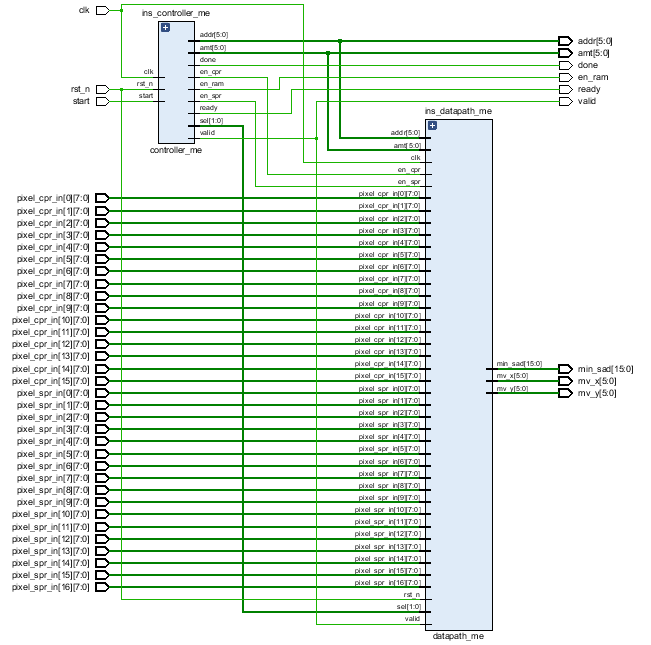
\includegraphics[width = 3in]{./Figures/mehardware.png}
	\rule{35em}{0.5pt}
	\caption{Schematic for inter-prediction module.}
	\label{fig:mehardware}
\end{figure}
\subsection{Resource Utilization}
The module for inter-prediction is analyzed and synthesized using Vivado for Xilinx Artix-7. The resource utilization for this module is shown below.
\begin{table}[H]
	\centering
	\begin{tabular}{|c|c|c|c|} \hline
		\textbf{Resource} & \textbf{Used} & \textbf{Available} & \textbf{Utilization\%}  \\ \hline
		Look Up Tables & 7376 & 63400 & 11.63 \\ \hline
		Registers & 7266 & 126800 & 5.73 \\ \hline
		Input/Output & 311 & 210 & 148.10 \\ \hline 
	\end{tabular}
	\caption{Resource utilization of inter-prediction module for Artix-7.}
	\label{tab:resource_me}
\end{table}

It can be seen from the results above that the utilization of look up tables and registers is within limits but the input/output has exceeded from the available resources. This issue is due to the fact that inter-prediction block has been synthesized separately. Once this module is integrated within the H.264 top module, the input/output ports will be reduced sufficiently.  

\subsection{Simulation Results}
In order to verify the working of inter-prediction module, it is simulated using a MB of size 16x16 from the current frame and a search range of size 48x48 from the reference frame.

The loading of MB takes 16 cycles and after that the pixels of search range are loaded in the RAMs. It takes 16 cycles to calculate the first valid SAD value as the RAMs are getting filled for the first time. Once the first valid SAD value is calculated the next values are calculated with no latency. This is due to the fact that RAMs are filled and only the shifting of pixels need to be done which is done by BRAM 16 as seen in figure \ref{fig:256pevbsme}. Therefore, this architecture reduces the latency for SAD calculation. This can also be verified by the following simulation waveform.
\begin{figure}[H]
	\centering
	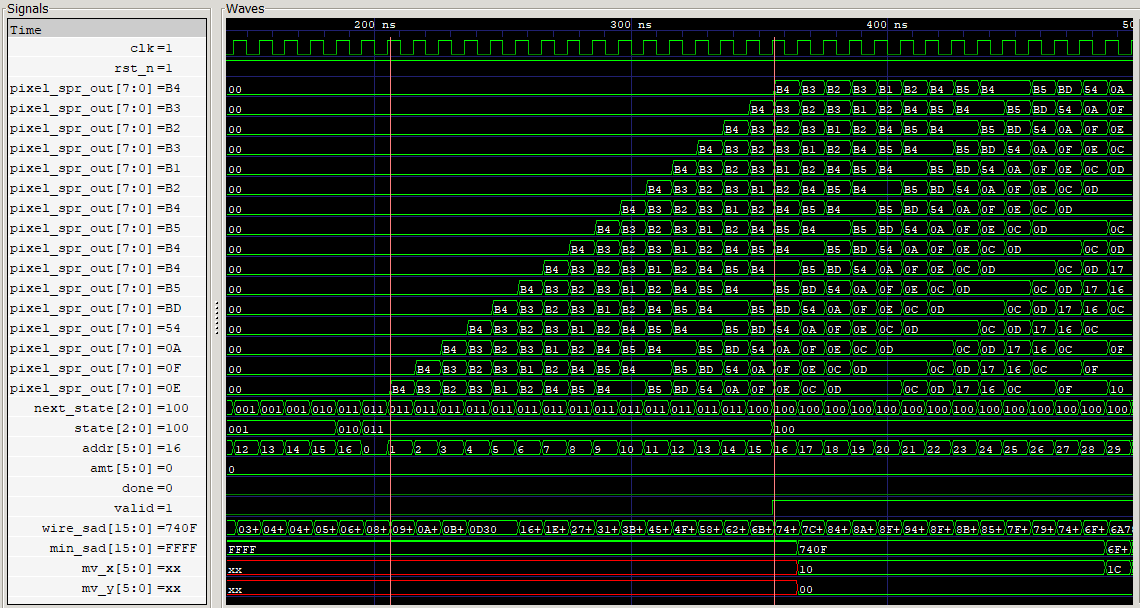
\includegraphics[width = 4in]{./Figures/wave3.png}
	\rule{35em}{0.5pt}
	\caption{Simulation waveform of inter-prediction module for one search range (a).}
	\label{fig:wave3}
\end{figure}
Once the MB has traversed the search range, it asserts a signal done and the final values for motion vectors in x and y direction, corresponding to the minimum SAD value are obtained. 
\begin{figure}[H]
	\centering
	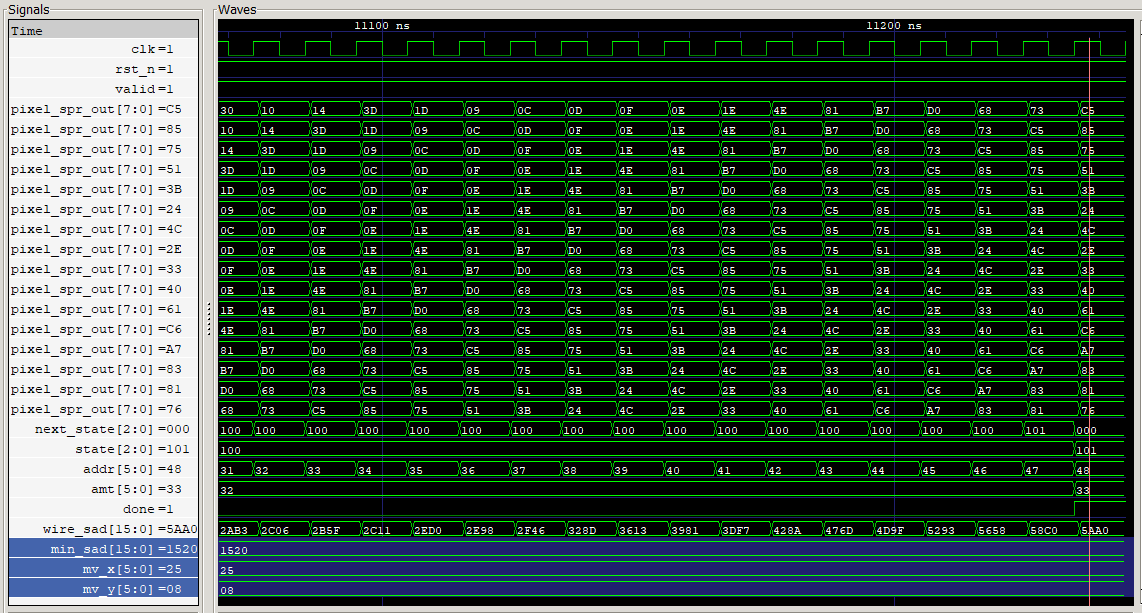
\includegraphics[width = 4in]{./Figures/wave2.png}
	\rule{35em}{0.5pt}
	\caption{Simulation waveform of inter-prediction module for one search range (b).}
	\label{fig:wave2}
\end{figure}

